
\documentclass[notheorems,serif]{beamer}

%选用主题
%\usetheme{Rochester}
%\usetheme{default}
%\usetheme{AnnArbor}
%\usetheme{Antibes}
%\usetheme{Bergen}
%\usetheme{Berkeley}
%\usetheme{Berlin}
%\usetheme{Boadilla}
%\usetheme{CambridgeUS}
%\usetheme{Copenhagen}
%\usetheme{Darmstadt}
%\usetheme{Dresden}
%\usetheme{Frankfurt}
%\usetheme{Goettingen}%
%\usetheme{Hannover}
%\usetheme{Ilmenau}
%\usetheme{JuanLesPins}
%\usetheme{Luebeck}
\usetheme{Madrid}
%\usetheme{Malmoe}
%\usetheme{Marburg}
%\usetheme{Montpellier}
%\usetheme{PaloAlto}
%\usetheme{Pittsburgh}
%\usetheme{Rochester}
%\usetheme{Singapore}
%\usetheme{Szeged}
%\usetheme{Warsaw}

% As well as themes, the Beamer class has a number of color themes
% for any slide theme. Uncomment each of these in turn to see how it
% changes the colors of your current slide theme.

%\usecolortheme{albatross}
%\usecolortheme{beaver}
%\usecolortheme{beetle}
%\usecolortheme{crane}
%\usecolortheme{dolphin}
%\usecolortheme{dove}
%\usecolortheme{fly}
%\usecolortheme{lily}
%\usecolortheme{orchid}
%\usecolortheme{rose}
%\usecolortheme{seagull}
%\usecolortheme{seahorse}
%\usecolortheme{whale}
%\usecolortheme{wolverine}

%设置被cover的内容不显示
%\setbeamercovered{transparent}

\useinnertheme{rounded}
\usecolortheme{default}

%调用包
\usepackage[no-math, cm-default]{fontspec}
\usepackage{xltxtra}
\usepackage{xunicode}   
\usepackage{xcolor}
\usepackage{amsmath,amssymb}
\usepackage{xeCJK}
\usepackage{multimedia}
\usepackage{listings}
\usepackage{subfigure}
\usepackage{todonotes}
\presetkeys{todonotes}{inline}{} 
\usepackage{multicol}
\usepackage{changes}




%将系统字体名映射为逻辑字体名称,主要是为了维护的方便  
\newcommand\fnhei{Adobe 黑体 Std}  
\newcommand\fnsong{Adobe 宋体 Std}  
\newcommand\fnkai{Adobe 楷体 Std}  
\newcommand\fnmono{DejaVu Sans Mono}  
\newcommand\fnroman{Times New Roman}  

\renewcommand{\normalsize}{\wuhao}

%%设置常用中文字号,方便调用  
\newcommand{\erhao}{\fontsize{22pt}{\baselineskip}\selectfont}  
\newcommand{\xiaoerhao}{\fontsize{18pt}{\baselineskip}\selectfont}  
\newcommand{\sanhao}{\fontsize{16pt}{\baselineskip}\selectfont}  
\newcommand{\xiaosanhao}{\fontsize{15pt}{\baselineskip}\selectfont}  
\newcommand{\sihao}{\fontsize{14pt}{\baselineskip}\selectfont}  
\newcommand{\xiaosihao}{\fontsize{12pt}{\baselineskip}\selectfont}  
\newcommand{\wuhao}{\fontsize{10.5pt}{\baselineskip}\selectfont}  
\newcommand{\xiaowuhao}{\fontsize{9pt}{\baselineskip}\selectfont}  
\newcommand{\liuhao}{\fontsize{7.5pt}{\baselineskip}\selectfont}  

%\setmainfont{\fnroman}
\setmainfont{\fnkai}
\setCJKmainfont[BoldFont=\fnhei]{\fnkai}  
\setCJKsansfont[BoldFont=\fnhei]{\fnkai}  
\setCJKmonofont{\fnkai}  

%楷体  
%\newfontinstance\KAI{\fnkai}  
%\newcommand{\kai}[1]{{\KAI#1}}  
%黑体  
%\newfontinstance\HEI{\fnhei}  
%\newcommand{\hei}[1]{{\HEI#1}}  
%英文  
%\newfontinstance\ENF{\fnroman}  
%\newcommand{\en}[1]{\,{\ENF#1}\,}

%楷体  
\newfontfamily\KAI {\fnkai}  
\newcommand{\kai}[1]{{\KAI#1}}  
%黑体  
\newfontfamily\HEI{\fnhei}  
\newcommand{\hei}[1]{{\HEI#1}}  
%英文  
\newfontfamily\ENF{\fnroman}  
\newcommand{\en}[1]{\,{\ENF#1}\,}


%连字符
\defaultfontfeatures{Mapping=tex-text}

%中文断行
\XeTeXlinebreaklocale "zh"
\XeTeXlinebreakskip = 0pt plus 1pt minus 0.1pt


%%%% 定理类环境的定义 %%%%
\newtheorem{example}{\hei{例子}} 
\newtheorem{problem}{\hei{问题}}           
\newtheorem{algorithm}{\hei{算法}}
\newtheorem{theorem}{\hei{定理}}
\newtheorem{definition}{\hei{定义}}
\newtheorem{axiom}{\hei{公理}}
\newtheorem{property}{\hei{性质}}
\newtheorem{proposition}{\hei{命题}}
\newtheorem{lemma}{\hei{引理}}
\newtheorem{corollary}{\hei{推论}}
\newtheorem{remark}{\hei{注解}}
\newtheorem{condition}{\hei{条件}}
\newtheorem{conclusion}{\hei{结论}}
\newtheorem{assumption}{\hei{假设}}

%重定义一些环境的名字
\renewcommand{\proofname}{\hei{证明}}
\renewcommand\tablename{\hei{表}}

%---SCRIPT-----------------------------------------------------------------------------------------
\newcommand{\cA}{\mathcal{A}}
\newcommand{\cB}{\mathcal{B}}
\newcommand{\cC}{\mathcal{C}}
\newcommand{\cD}{\mathcal{D}}
\newcommand{\cE}{\mathcal{E}}
\newcommand{\ce}{\mathcal{e}}
\newcommand{\cF}{\mathcal{F}}
\newcommand{\cG}{\mathcal{G}}
\newcommand{\cg}{\mathcal{g}}
\newcommand{\cH}{\mathcal{H}}
\newcommand{\cI}{\mathcal{I}}
\newcommand{\cJ}{\mathcal{J}}
\newcommand{\cK}{\mathcal{K}}
\newcommand{\cL}{\mathcal{L}}
\newcommand{\cM}{\mathcal{M}}
\newcommand{\cN}{\mathcal{N}}
\newcommand{\cO}{\mathcal{O}}
\newcommand{\cP}{\mathcal{P}}
\newcommand{\cQ}{\mathcal{Q}}
\newcommand{\cR}{\mathcal{R}}
\newcommand{\cS}{\mathcal{S}}
\newcommand{\cT}{\mathcal{T}}
\newcommand{\cU}{\mathcal{U}}
\newcommand{\cV}{\mathcal{V}}
\newcommand{\cW}{\mathcal{W}}
\newcommand{\cX}{\mathcal{X}}
\newcommand{\cY}{\mathcal{Y}}
\newcommand{\cZ}{\mathcal{Z}}
\newcommand{\cz}{\mathcal{z}}
%---BLACKBOARD-------------------------------------------------------------------------------------
\newcommand{\mA}{\mathbb A}
\newcommand{\mB}{\mathbb B}
\newcommand{\mC}{\mathbb C}
\newcommand{\mD}{\mathbb D}
\newcommand{\mE}{\mathbb E}
\newcommand{\mF}{\mathbb F}
\newcommand{\mG}{\mathbb G}
\newcommand{\mg}{\mathbb g}
\newcommand{\mH}{\mathbb H}
\newcommand{\mI}{\mathbb I}
\newcommand{\mJ}{\mathbb J}
\newcommand{\mK}{\mathbb K}
\newcommand{\mL}{\mathbb L}
\newcommand{\mM}{\mathbb M}
\newcommand{\mN}{\mathbb N}
\newcommand{\mO}{\mathbb O}
\newcommand{\mP}{\mathbb P}
\newcommand{\mQ}{\mathbb Q}
\newcommand{\mR}{\mathbb R}
\newcommand{\mS}{\mathbb S}
\newcommand{\mT}{\mathbb T}
\newcommand{\mU}{\mathbb U}
\newcommand{\mV}{\mathbb V}
\newcommand{\mW}{\mathbb W}
\newcommand{\mX}{\mathbb X}
\newcommand{\mY}{\mathbb Y}
\newcommand{\mZ}{\mathbb Z}
\newcommand{\mz}{\mathbb z}

\newcommand{\bV}{\mathbf{V}}
\newcommand{\bz}{\mathbf{z}}
\newcommand{\bT}{\mathbf{T}}
\newcommand{\bx}{\mathbf{x}}
\newcommand{\be}{\mathbf{e}}
\newcommand{\bff}{\mathbf{f}}
\newcommand{\bg}{\mathbf{g}}
\newcommand{\bn}{\mathbf{n}}
\newcommand{\bt}{\mathbf{t}}
\newcommand{\bd}{\mathbf{d}}
\newcommand{\bzero}{\mathbf{0}}
\newcommand{\bka}{\mathbf{\kappa}}

\newcommand{\rd}{\mathrm{d}}
%---SHORTCUTS--------------------------------------------------------------------------------------
\newcommand\xor{\mathbin{\char`\^}}
\DeclareMathOperator{\res}{Res}
\DeclareMathOperator{\sgn}{sgn}
\DeclareMathOperator{\supp}{supp}
\DeclareMathOperator{\as}{as}
\newcommand{\slant}[1]{\slshape #1\normalfont}
\newcommand{\dd}[2]{\frac{d#1}{d#2}} 
\newcommand{\ddx}{\frac{d}{dx}}
\newcommand{\ddt}{\frac{d}{dt}}
\newcommand{\dds}{\frac{d}{ds}}
\newcommand{\pd}[1]{\ds\frac{\partial}{\partial #1 }}
\newcommand{\pdd}[2]{\ds\frac{\partial #1}{\partial #2 }}
\newcommand{\mdd}[3]{\ds\frac{\partial^{#3} #1}{\partial #2^{#3} }}
\newcommand{\x}{\ _\Box}
\newcommand{\ds}{\displaystyle}
\newcommand{\bs}{\backslash}
\newcommand{\Bold}{\noindent \bfseries}
\newcommand{\Norm}{\normalfont}
\newcommand{\exl}[1]{\textcolor{NavyBlue}{\Bold Exercise #1 \Norm}}
\newcommand{\ex}{\textcolor{NavyBlue}{\Bold Problem: \Norm}}
\newcommand{\sol}{\textcolor{Mulberry}{\Bold Solution: \Norm}}
\newcommand{\pf}{\textcolor{Mulberry}{\Bold Proof: \Norm}}
\newcommand{\Title}[1]{\LARGE\Bold \textcolor{Sepia}{#1}\Norm\normalsize \vspace{10pt} \newline}
\newcommand{\prop}{\Bold \textcolor{YellowOrange}{ Proposition:} \Norm}
\newcommand{\propl}[1]{\Bold \textcolor{YellowOrange}{ Proposition #1:} \Norm}
\newcommand{\rk}{\Bold \textcolor{YellowOrange}{ Remark:} \Norm}
\newcommand{\rmk}[1]{\Bold\textcolor{YellowOrange}{#1} \Norm}
\newcommand{\thm}[1]{\Bold \textcolor{YellowOrange}{ Theorem #1} \Norm}
\newcommand{\ind}{\indent\indent}
\newcommand{\br}{\vspace{10pt} \newline}

\newcommand{\red}{\color{red}}
\newcommand{\blue}{\color{blue}}



\usepackage{amsmath}

\allowdisplaybreaks[4]

\begin{document}

	\title[数值线性代数]
	
	\institute[湘潭大学数学系]
	
	\date[\today]
	
	
	\AtBeginSection[]{
		
		\frame<beamer>{ 
			
			\frametitle{第五讲~~对称矩阵的特征值问题}   
			
			\tableofcontents[currentsection] 
			
		}
	}
\section{Jacobi迭代}
\begin{frame}
关于对称特征值问题的常用算法有(直接法):
$\bullet$ \textcolor{blue}{Jacobi迭代}:最古老,收敛速度较慢,但精度较高,且很适合并行计算。
$\bullet$ \textcolor{blue}{Rayleigh商迭代}:一般具有三次收敛性,但需要解方程组。
$\bullet$ \textcolor{blue}{对称QR迭代}:对称矩阵的QR方法.对于对称三对角矩阵,若只计算特征值,则速
	度最快(运算量为$\mathcal O(n^2)$)。如果还需要计算特征向量,则运算量约为$6n^3$。
$\bullet$ \textcolor{blue}{分而治之法}:同时计算特征值和特征向量的一种快速算法。基本思想时将大
	矩阵分解形成小矩阵,然后利用递归思想求特征值。在最坏的情形下,运算量为
	$\mathcal O(n^3)$。在实际应用中,平均为$\mathcal O(n^{2.3})$。如果使用快速多
	极子算法(FMM)后,理论上的运算量可降低到$\mathcal O(nlog^p n)$,其中$p$时一个
	较小的整数,这使得分而治之算法陈给目前计算对称三对角矩阵的 \textcolor{blue}{特征
		值和特征向量}的
	首选方法。
\end{frame}
\begin{frame}
$\bullet$ \textcolor{blue}{对分法和反迭代}:对分法主要用于求解对称三交矩阵在某个区间中的特征
	值,运算量约为$\mathcal O(kn)$。其中$k$为所需计算的特征值的个数。反迭代用于计
	算特征向量,在最佳情况下,即特征值“适当分离”时,运算量约为$\mathcal O(kn)$,
	但在最差情况下,即特征值成串的紧靠在一起时,运算量约为$\mathcal O(k^2n)$,而
	且不能保证特征向量的精度(虽然实际上它几乎是精确的)。


\qquad 除了Jacobi迭代和Rayleigh商迭代外,其余算法都需要先将对称矩阵三对角化,这个过程大
约需花费$\frac{4}{3} n^3$的工作量,如果需要计算特征向量的话,则运算量约为
$\frac{8}{3}n^3$。
\end{frame}
\begin{frame}
\frametitle{1\qquad Jacobi迭代}

\textcolor{blue}{基本思想}\quad 通过一系列的 \textcolor{blue}{Jacobi旋转}将A正交相似于一个对角矩阵:
$$A^{(0)}=A,A{(K+1)}=J_k^TA^{(k)}J_k,k=0,1,\cdots,$$
且$A{(0)}$收敛到一个对角矩阵,其中$J^k$为Jacobi旋转,即Givens变换:

\begin{figure}[H]
	\centering
	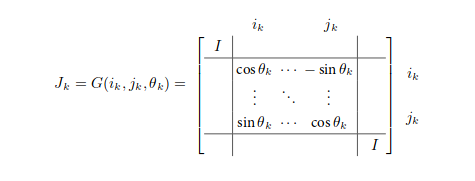
\includegraphics[scale=0.7]{figurest/figure_1.png}
\end{figure}
\end{frame}
\begin{frame}
\textcolor{blue}{引理}\quad 设$A\in\mathbb{R}^{2\times 2}$是对角矩阵。则存在Givens变换$G\in \mathbb{R}^{2\times 2}$使得$G^TAG$为对角阵。
\end{frame}
\begin{frame}
为了使$A^{(K)}$收敛到一个对角矩阵,其非对角素必须趋向于0。

记$off(A)$为所有非对角元素的平方和,即
$$off(A)=\sum_{i\neq j}a_{ij}^2=\|A^2\|_F^2-\sum_{i=1}^na_{ii}^2$$

我们的目标就是使得$off(A)$尽快趋向于0。

\textcolor{blue}{引理}\quad 设$A=[a_{ij}]_{n\times n}\in \mathbb{R}^{n\times n}$
是对称矩阵。$\widehat{A}=[a_{ij}]_{n\times n}=J^TAJ$,$J=G(i.j,\theta)$,其中
$\theta$的选取使得$\widehat a_{ij}=\widehat a_{ji}=0$,则$$off(\widehat
A)=off(A)-2a_{ij}^2$$
\end{frame}
\begin{frame}
\textcolor{blue}{算法\quad1.1}\quad Jacobi迭代算法
\begin{enumerate}[1:]
	\item Given a symmetric matrix $A\in \mathbb R^{n\times n}$
	\item if eigenvectors are desired then
	\item \quad set $J=I$ and $shift=1$
	\item end if
	\item while not converge do
	\item \quad choose an index pair $(i,j)$such that $a_{ij}\neq 0$
	\item \quad $\tau=(a_{ii}-a_{jj})/(2a-{jj})$
	\item \quad $t=sign(\tau/(|\tau|+\sqrt{1+\tau ^2})$
	\item \quad $c=1/\sqrt{1+t^2},s=c\cdot t$
	\item \quad $A=G(i,j,\theta)^TAG(i,j,\theta)$
	\item \quad if $shift=1$ then 
	\item \qquad $J=J\cdot G(i,j,\theta)$
	\item \quad end if
	\item end while
\end{enumerate}
\end{frame}
\begin{frame}
\frametitle{$a_{ij}$的选取问题}



\qquad 一种直观的选取方法就是使得$a_{ij}$为所有非对角元素中绝对值最大的一个,这就是经典
Jacobi算法。\\
\end{frame}
\begin{frame}

\textcolor{blue}{算法\quad1.2}\quad 经典Jacobi迭代算法
\begin{enumerate}[1:]
	\item Given a symmetric matrix $A\in \mathbb R^{n\times n}$  
	\item if eigenvectors are desired then  
	\item \quad set $J=I$ and $shift=1$  
	\item end if  
	\item while $off(A)>tol $ do
	\item \quad choose $(i,j)$such that $a_{ij}=max_{k\neq l}|a_{kl}|$  
	\item \quad $\tau=(a_{ii}-a_{jj})/(2a-{jj})$  
	\item \quad $t=sign(\tau/(|\tau|+\sqrt{1+\tau ^2})$  
	\item \quad $c=1/\sqrt{1+t^2},s=c\cdot t$  
	\item \quad $A=G(i,j,\theta)^TAG(i,j,\theta)$  
	\item \quad if $shift=1$ then   
	\item \qquad $J=J\cdot G(i,j,\theta)$  
	\item \quad end if  
	\item end while  
\end{enumerate}  
\end{frame}
\begin{frame}

可以证明,经典Jacobi算法至少是线性收敛的。\\
\textcolor{blue}{定理}\quad 经典Jacobi算法\textcolor{blue}{1.2},有$$off(A^{(k+1)}) \le \left(1-\cfrac{1}{N} \right)\mathcal O(off(A^{(k)}),N=\cfrac{n(n-1)}{2}$$
故$k$步迭代后,有$$off(A^{(k+1)}) \le \left(1-\cfrac{1}{N} \right)^k \mathcal O(off(A^{(0)})=\left(1-\cfrac{1}{N} \right)^k \mathcal O(off(A)$$
\end{frame}
\begin{frame}

事实上,经典Jacobi算法最终是二次局部收敛的。
\textcolor{blue}{定理}\quad 经典Jacobi算法\textcolor{blue}{1.2}是N步局部二次收敛
的,即对足够大的$k$,有$$off(A^{(k+N)})=\mathcal O(off^2(A^{(k)})$$

\textcolor{blue}{循环Jacobi}\quad 经典Jacobi算法的每一步都要寻找绝对值最大的
非对角元,费时不实用。改进:逐行扫描。\\
\end{frame}
\begin{frame}

\textcolor{blue}{算法\quad1.3}\quad 经典Jacobi迭代算法(逐行扫描)
\begin{enumerate}[1:]
	\item Given a symmetric matrix $A\in \mathbb R^{n\times n}$
	\item if eigenvectors are desired then
	\item \quad set $J=I$ and $shift=1$
	\item end if
	\item while $off(A)>tol$ do
	\item \quad for $i=1$ to $n-1$ do
	\item \qquad for$j=i+1$ to $n$ do
	\item \qquad \quad if $a_{ij}\neq 0$ then
	\item \qquad \qquad $\tau=(a_{ii}-a_{jj})/(2a-{jj})$
	\item \qquad \qquad $t=sign(\tau/(|\tau|+\sqrt{1+\tau ^2})$
	\item \qquad \qquad $c=1/\sqrt{1+t^2},s=c\cdot t$
	\item \qquad \qquad $A=G(i,j,\theta)^TAG(i,j,\theta)$
	\item \qquad \qquad if $shift=1$ then
	\item \qquad \qquad \quad$J=J\cdot G(i,j,\theta)$
	\item \qquad \qquad end if
	\item \qquad \quad end if
	\item \qquad end for
	\item \quad end for
	\item end while
\end{enumerate}

循环Jacobi也具有局部二次收敛性。
\end{frame}
\section{Raylaogh商迭代}
\begin{frame}
\frametitle{2\qquad Raylaogh商迭代}



反迭代方法中,以Rayleigh商作为位移。

关于Rayleigh商迭代的收敛性,我们有下面的结论。

\textcolor{blue}{定理}\quad 设$A\in \mathbb R^{n\times n}$对称,且特征值都是单
重的。则当误差足够小时,Rayleigh商迭代中每步迭代所得的正确数字的位数曾至三倍,即
Rayleigh商迭代是局部三次收敛。
\end{frame}
\section{对称QR迭代}
\begin{frame}
\frametitle{3\qquad 对称QR迭代}


将带位移的隐式QR方法运用到对称矩阵,就得到对称QR迭代方法。
基础步骤:
\begin{enumerate}[1.]
	\item 对称三对角化:利用Householder变换,将$A$化为对称三对角矩阵,即计算正交
	矩阵$Q$使得$T=QAQ^T$为对称三对角矩阵;
	\item 使用带(单)位移的隐式QR迭代算法计算T的特征值与特征向量;
	\item 计算$A$的特征向量。
\end{enumerate}
\end{frame}
\begin{frame}
对称三对角化

任何一个对称矩阵$A\in \mathbb R^{n\times n}$都可以通过正交变换转化成一个对称三对
角矩阵$T$。这个过程可以通过Householder变换来实现,也可以通过Givens变换来实现。\\
对称QR迭代算法的运算量
\begin{itemize}
	\item[$\bullet$] 三对角化$4n^3/3+\mathcal O(n^2)$,若需计算特征向量,则为
	$8n^3/3+\mathcal O(n^2)$;
	\item[$\bullet$] 对$T$做带位移的隐式QR迭代,每次迭代的运算量为$6n$;
	\item[$\bullet$] 计算特征值,假定每个平均迭代2步,则总运算量为
	$12n^2$;
	\item[$\bullet$] 若要计算$T$的所有特征值和特征向量,则运算量为$6n^3+\mathcal
	O(n^2)$;
	\item[$\bullet$] 若只要计算A的所有特征值,运算量为$4n^3/3+\mathcal O(n^2)$;
	\item[$\bullet$] 若计算$A$的所有特征值和特征向量,则运算量为
	$26n^3/3+\mathcal O(n^2)$;
\end{itemize}
\end{frame}
\begin{frame}
\frametitle{位移的选取——Wilkinson位移}


位移的好坏直接影响到算法的收敛速度。我们可以通过下面的方式来选取位移。设
$$A^{(k)}=\begin{bmatrix}
a_1^{(k)}&b_1^{(k)}&&\\
b_1^{(k)}&\ddots &\ddots &\\
&\ddots &\ddots &b_{n-1}^{k}\\
&&b_{n-1}^{(k)}&a_n^{(k)}
\end{bmatrix}$$

一种简单的位移选取策略就是令$\sigma _k=a_n{(K)}$。事实上,$a_n^{(k)}$就是收敛到
特征向量的迭代向量的Rayleigh商。这种位移选取方法几乎对所有的矩阵都有三次渐进收敛速度。但也存在不收敛的例子,故我们需要对其做改进。
\end{frame}
\begin{frame}

\textcolor{blue}{Wilkinson位移:}取$\begin{bmatrix}a_{n-1}^{(k)}&b_{n-1}^{(k)}\\
b_{n-1}^{(k)}&a_n^{(k)} \end{bmatrix}$的最接近$a_n^{(k)}$的特征值作为位移。通过
计算可得Wilkinson位移为
$$\sigma =a_n^{(k)}+\delta -sign(\delta)\sqrt{\delta
	^2+(b_{n-1}^{(k)})^2}$$,
其中$\delta=\
frac{1}{2}(a_{n-1}^{(k)}-a_n^{(K)})$
出于稳定性方面的考虑,我们通常用下面的计算公式\begin{equation}
\sigma=a_n^{(k)}-\cfrac{(b_{n-1}{(k)})^2}{\delta +sign(\delta)\sqrt{\delta
		^2+(b_{n-1}^{(k)})^2}}
\end{equation}

\textcolor{blue}{定理}\quad 采用Wilkinson位移的QR迭代时整体收敛的,且至少是线性收敛。事实上,几乎所有的矩阵都是渐进三次收敛的。
\end{frame}
\begin{frame}
\textcolor{blue}{例}\quad 带Wilkinson位移的隐式QR迭代算法收敛性演示。

MATLAB代码:$Eig_TriQR.m$
\end{frame}
\section{分而治之法}
\begin{frame}
\frametitle{4\qquad 分而治之法}

分而治之法由Cuppen于1981年首次提出,但直到1995年才出现稳定的实现方式,是目前计算\textcolor{blue}{所有特征值和特征向量}的最快算法。\\
考虑不可约对称三对角矩阵
\begin{figure}
	\begin{center}
		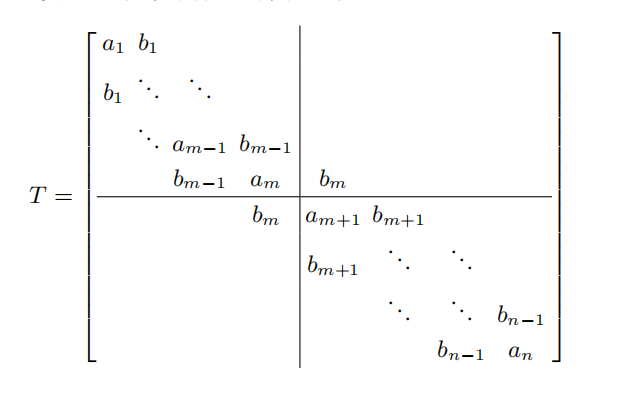
\includegraphics[scale=0.5]{figurest/figure_4.png}
	\end{center}
\end{figure}
\end{frame}
\begin{frame}
\begin{figure}
	\begin{center}
		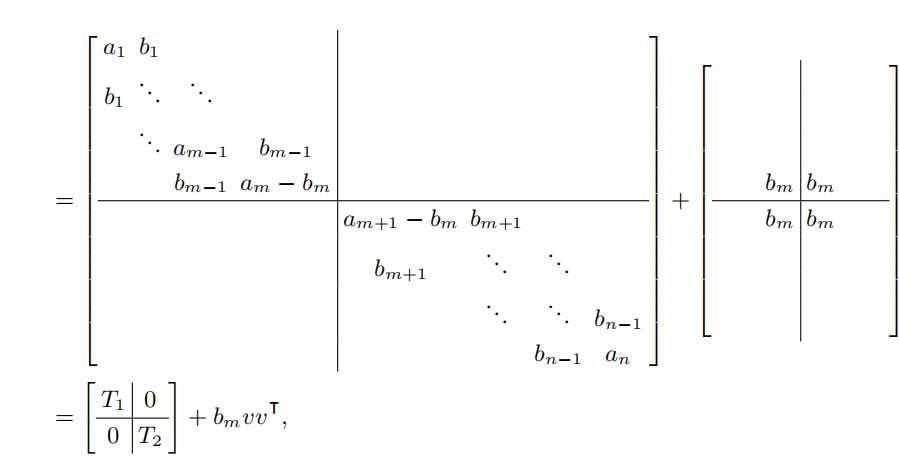
\includegraphics[scale=0.39]{figurest/figure_5.png}
	\end{center}
\end{figure}
其中$v=[0,\cdots ,0,1,1,0,\cdots ,0]^T$。
\end{frame}
\begin{frame}
\frametitle{假定$T_1$和$T_2$的特征值已经计算出来}
即$T_1=Q_1\boldsymbol{\Lambda}_1Q_1^T$,$T_2=Q_2\boldsymbol{\Lambda}_2Q_2^T$,下面考虑$T$的特征值分解。
$$
\begin{aligned} T=\left[\begin{array}{cc}{T_{1}} & {0} \\ {0} & {T_{2}}\end{array}\right]+b_{m} v v^{\mathrm{T}} &=\left[\begin{array}{cc}{Q_{1} \Lambda_{1} Q_{1}^{\mathrm{T}}} & {0} \\ {0} & {Q_{2} \Lambda_{2} Q_{2}^{\mathrm{T}}}\end{array}\right]+b_{m} v v^{\mathrm{T}} \\ &=\left[\begin{array}{cc}{Q_{1}} & {0} \\ {0} & {Q_{2}}\end{array}\right]\left(\left[\begin{array}{cc}{\Lambda_{1}} & {0} \\ {0} & {\Lambda_{2}}\end{array}\right]+b_{m} u u^{\mathrm{T}}\right)\left[\begin{array}{cc}{Q_{1}} & {0} \\ {0} & {Q_{2}}\end{array}\right]^{\top} \end{aligned}
$$
其中$$
u=\left[\begin{array}{cc}{Q_{1}} & {0} \\ {0} & {Q_{2}}\end{array}\right]^{\top}
,v=\left[\begin{array}{c}
Q_1^T\mbox{的最后一列}\\Q_2^T\mbox{的第一列}
\end{array}\right]$$

令$a=b_m$,$D=diag(\Lambda_1,\Lambda_2)=diag(d_1,d_2,\cdots ,d_n)$,并假定$d_1\ge d_2\ge \cdots \ge d_n$,则$T$的特征值于$D+\alpha uu^T$的特征值相同。
\end{frame}
\begin{frame}
\frametitle{考虑$D+\alpha uu^T$的特征值}


设$\lambda$是$D+\alpha uu^T$的一个特征值,若$D-\lambda I$非奇异,则$$det(D+\alpha uu^T-\lambda I)=det(D-\lambda I)\cdot det(I+\alpha(D-\lambda I)^{-1}uu^T)$$
故$det(D+\alpha uu^T-\lambda I)=0$。

\textcolor{blue}{引理}\quad 设$x,y\in \mathbb R^n$,则$det(I+xy^T)=1+y^Tx$。

于是$$det(I+\alpha(D-\lambda I)^{-1}uu^T)=1+\alpha u^T(D-\lambda I)^{-1}u=1+\alpha \sum_{i=1}^{n}\cfrac{u_i^2}{d_i-\lambda} \triangleq f(\lambda)$$
故求$A$的特征值等价于求特征方程$f(\lambda)=0$的根。\\
\end{frame}
\begin{frame}
由于$$f'(\lambda)=\alpha \sum_{i=1}^{n}\cfrac{u_i^2}{(d_i-\lambda)}$$

当所有的$d_i$都互不相同,且所有的$u_i$都不为零时,$f(\lambda)$在$\lambda \neq d_i$处都是严格单调的。
\begin{figure}[H]
	\centering
	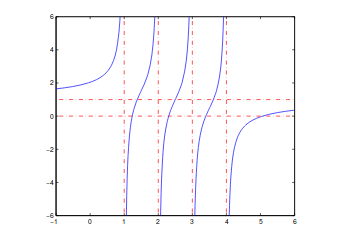
\includegraphics[scale=0.6]{figurest/figure_2.png}
\end{figure}
\end{frame}
\begin{frame}
所以$f(\lambda)$在每隔区间$(d_{i+1},d_i)$内都有一个根,共$n-1$个,另一个根在$(d_1,\infty)$(若$\alpha >0$)或($-\infty,d_n$)若$\alpha <0$)中。

由于$f(\lambda)$在每个区间$(d_{i+1},d_i)$内光滑且严格单调递增($\alpha >0$)或递减($\alpha <0$),所以在实际计算中,可以使用对分法,牛顿法及其变形,或有理逼近等算法求解。通常都很快收敛,一般只需迭代几步即可。

因此,计算一个特征值的运算量约为$\mathcal{O}(n)$,计算$D+\alpha\ uu^T$的所有特征向量。

\textcolor{blue}{引理}\quad 设$D\in \mathbb R^{n\times n}$为对角矩阵,$u\in \mathbb R^n$,$\alpha \in \mathbb R$,若$\lambda$是$D+\alpha\ uu^T$的特征值,且$\lambda \neq d_i$,$i=1,2,\cdots ,n$,则$(D-\lambda I)^{-1}u$是其对应的特征向量。\\
\end{frame}
\begin{frame}
\textcolor{blue}{算法 4.1}\quad 计算对称三对角矩阵的特征值和特征向量的分而治之法
\begin{enumerate}[1:]
	\item function $[Q,\Lambda]=dc\_eig(T)$  \quad $\%T=Q\Lambda Q^T$
	\item if $T$is of $1\times 1$then
	\item \quad $Q=1$,$\Lambda=T$
	\item \quad return
	\item end if
	\item form $T=\left[\begin{array}{cc}{T_{1}} & {0} \\ {0} & {T_{2}}\end{array}\right]+b_{m} v v^{\top}
	$
	\item $\left[Q_{1}, \Lambda_{1}\right]=\mathrm{d} c_{-} \operatorname{eig}\left(T_{1}\right)$
	\item $\left[Q_{2}, \Lambda_{2}\right]=\mathrm{d} c_{-} \operatorname{eig}\left(T_{2}\right)$
	\item form $D+\alpha uu^T$from$\Lambda_{1},\Lambda_{2},Q_1,Q_2$
	\item compute the eigenvalues $\Lambda$and eigenvectors  $\hat{Q}$ of $D+\alpha uu^T$
	\item compute the eigenvalues of $T$ with $Q=\left[\begin{array}{cc}{Q_{1}} & {0} \\ {0} & {Q_{2}}\end{array}\right] \cdot \hat{Q}$
	\item end
\end{enumerate}
\end{frame}
\begin{frame}
在分而治之法中,计算特征值和计算特征向量是同时进行的。
\end{frame}
\begin{frame}
下面我们详细讨论分而治之算法的几个细节问题:
\begin{enumerate}[(1)]
	\item 如何减少运算量;
	\item 如何求解特征方程$f(\lambda)=0$;
	\item 如何稳定的计算特征向量。
\end{enumerate}
\end{frame}
\begin{frame}
\frametitle{(1)如何减小运算量——收缩技巧(deflation)}

分而治之算法的计算复杂性分析如下:用$t(n)$表示对$n$阶矩阵调用函数$dc\_eig$的运算量,则
\begin{equation*}
	\begin{aligned}
		t(n)=&2t(n/2)\qquad \mbox{递归调用}dc_eig\mbox{两次}\\&+\mathcal{O}(n^2)\qquad  \mbox{计算}D+\alpha uu^T \mbox{的特征值和特征向量}\\&+c\cdot n^3 \qquad \mbox{计算}Q
	\end{aligned}
\end{equation*}

如果计算$Q$时使用的是稠密矩阵乘法,则$c=2$;若不计$\mathcal{O} (n^2)$项,则由递归公式$t(n)=2t(n/2)+c\cdot n^3$可得$t(n)\thickapprox c\cdot 4n^3/3$。

但事实上,由于收缩现象的存在,常熟$c$通常比1小得多。
\end{frame}
\begin{frame}
在前面的算法描述过程中,我们假定$d_i$互不相等且$u_i$不能等于零。

事实上,当$d_i=d_{i+1}$或$u_i=0$时,$d_i$即为$D+\alpha uu^T$的特征值,这种现象我们成为收缩。

在实际计算时,当$d_i-d_{i+1}$或$|u_i|$小于一个给定的阈值时,我们就金斯认为$d_i$为$D+\alpha uu^T$的特征值,即出现收缩现象。

在实际计算中,收缩现象会经常发生,而且会非常频繁,所以我们可以而且应该利用这种有点加快分而治之算法的速度。

由于主要的计算量集中在计算$Q$,即算法的最后一步的矩阵的乘积。如果$u_i=0$,则$d_i$为特征值,其对应的特征向量$e_i$,即$\hat{Q}$的第$i$列为$e_i$,故计算$Q$的第$i$列时不需要做任何的计算。

当$d_i=d_{i+1}$时,也存在一个类似的简化。\\
\end{frame}
\begin{frame}
\frametitle{(2)特征方程求解}


通常我们可以使用牛顿法来计算特征方程$f(\lambda)=0$的解。当$d_i\neq d_{i+1}$且$u_i\neq 0$时,用牛顿法计算$f(\lambda)$在$(d_{i+1},d_i)$中的零点$\lambda _i$。如果$|u_i|$小于给定的阈值时,我们可直接将$d_i$作为特征值$\lambda _i$的一个近似。但当$u_i$很小(却大于给定的阈值)时,此时$f(\lambda)$在区间$[d_{i+1},d_i]$中的大部分处的斜率几乎为0(见下图)。这是,如果任取$[d_{i+1},d_i]$中的一个点作为迭代初始点,经过一次牛顿迭代后,迭代解可能会跑到区间$[d_{i+1},d_i]$的外面,造成不收敛。
\begin{figure}[H]
	\centering
	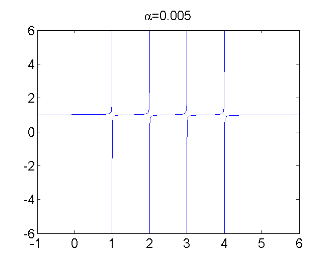
\includegraphics[scale=0.4]{figurest/figure_3.png}
	\caption{$f(\lambda)=1+0.005(\cfrac{1}{4-\lambda}+\cfrac{1}{3-\lambda}+\cfrac{1}{2-\lambda}+\cfrac{1}{1-\lambda})$的图像}
\end{figure}
\end{frame}
\begin{frame}
这时需要采用修正的牛顿法。假设我们已经计算出$\lambda _i$的一个近似$\tilde{\lambda}$,下面我们需要从$\tilde{\lambda}$出发,利用牛顿迭代计算下一个近似,直至收敛。我们知道牛顿法的基本原理是使用$f(\lambda)$在点$\tilde{\lambda}$的切线来近似$f(\lambda)$,并将切线的零点作为下一个近似,即用直线来近似曲线$f(\lambda)$。

当$u_i$很小时,这种近似方法会出现问题,此时不能使用直线来近似$f(\lambda)$。这时我们可以寻找其他简单函数$h(\lambda)$来近似$f(\lambda)$,然后用$h(\lambda)$的零点作为$f(\lambda)$零点的近似,并不断迭代下去,直至收敛。

当然,$h(\lambda)$需要满足一定的要求:
\begin{enumerate}[(1)]
	\item 必须容易构造;
	\item 其零点容易计算;
	\item 尽可能与$f(\lambda)$相近。
\end{enumerate}
\end{frame}
\begin{frame}

下面给出构造$h(\lambda)$的一种方法。

因为$d_i$和$d_{i+1}$是$f(\lambda)$的奇点,所以我们令$$h(\lambda)=\cfrac{c_1}{d_i-\lambda}+\cfrac{c_2}{d_{i+1}-\lambda}+c_3$$
其中$c_1,c_2,c_3$为参数。显然,$h(\lambda)$的零点很容易计算(与Newton法相差无几)。在选取这些参数时,要使得$h(\lambda)$在$\tilde{\lambda}$附近尽可能地接近$f(\lambda)$。记$$\begin{aligned}
f(\lambda)=1+\alpha \sum_{k=1}^n \cfrac{u_k^2}{d_k-\lambda}&=1+\alpha (\sum_{k=1}^i \cfrac{u_k^2}{d_k-\lambda}+1+\alpha \sum_{k=i+1}^n \cfrac{u_k^2}{d_k-\lambda})\\&\triangleq 1+\alpha\left(\Psi_{1}(\lambda)+\Psi_{2}(\lambda)\right)
\end{aligned}$$

当$\lambda \in (d_{i+1},d_i)$时,$\Psi_{1}(\lambda)$为正项和,$\Psi_{2}(\lambda)$为负项的和,因此它们都可以较精确地计算。但如果把它们加在一起时可能会引起对消,从而失去相对精度。因此我们也将$h(\lambda)$写成$$h(\lambda)=1+\alpha(h_1(\lambda)+h_2(\lambda))$$
\end{frame}
\begin{frame}

其中$$
h_{1}(\lambda)=\frac{c_{1}}{d_{i}-\lambda}+\hat{c}_{1}, \quad h_{2}(\lambda)=\frac{c_{2}}{d_{i+1}-\lambda}+\hat{c}_{2}
$$
满足$$
\begin{aligned} h_{1}(\tilde{\lambda}) &=\Psi_{1}(\tilde{\lambda}), \quad h_{1}^{\prime}(\tilde{\lambda})=\Psi_{1}^{\prime}(\tilde{\lambda}) \\ h_{2}(\tilde{\lambda}) &=\Psi_{2}(\tilde{\lambda}), \quad h_{2}^{\prime}(\tilde{\lambda})=\Psi_{2}^{\prime}(\tilde{\lambda}) \end{aligned}
$$
即$h_{1}(\lambda)$和$h_{2}(\lambda)$分别在点$\tilde{\lambda}$与$\Psi_{1}(\lambda)$和$\Psi_{2}(\lambda)$相切。这在数值插值中是常见的条件。容易计算可得\begin{equation}
\left\{\begin{array}{ll}{c_{1}=\Psi_{1}^{\prime}(\tilde{\lambda})\left(d_{i}-\tilde{\lambda}\right)^{2},} & {\hat{c}_{1}=\Psi_{1}(\tilde{\lambda})-\Psi_{1}^{\prime}(\tilde{\lambda})\left(d_{i}-\tilde{\lambda}\right)} \\ {c_{2}=\Psi_{2}^{\prime}(\tilde{\lambda})\left(d_{i+1}-\tilde{\lambda}\right)^{2},} & {\hat{c}_{2}=\Psi_{2}(\tilde{\lambda})-\Psi_{2}^{\prime}(\tilde{\lambda})\left(d_{i+1}-\tilde{\lambda}\right)}\end{array}\right.
\label{equation5.3}
\end{equation}
所以,最后取\begin{equation}
h(\lambda)=1+\alpha\left(\hat{c}_{1}+\hat{c}_{2}\right)+\alpha\left(\frac{c_{1}}{d_{i}-\lambda}+\frac{c_{2}}{d_{i+1}-\lambda}\right)
\label{equation5.4}
\end{equation}
这就是迭代函数。
\end{frame}
\begin{frame}
\textcolor{blue}{算法 4.2}\quad 修正的Newton算法
\begin{enumerate}[1:]
	\item set$k=0$
	\item choose an initial guess $\lambda _0\in [d_{i+1},d_i]$
	\item while not convergence do
	\item \quad let$\tilde{\lambda}=\lambda _k$and compute $c_1,c_2,\hat{c}_{1},\hat{c}_{2}$from \ref{equation5.3}
	\item \quad set $k=k+1$
	\item \quad compute the solution $\lambda _k$of $h(\lambda)$defined by \ref{equation5.4}
	\item end while
\end{enumerate}
\end{frame}
\begin{frame}
\frametitle{(3)计算特征向量的稳定算法}


设$\lambda_i$是$D+\alpha uu^T$的特征值,则根据引理4.2,可利用公式$\left(D-\lambda_{i} I\right)^{-1} u$来计算其对应的特征向量。但遗憾的是,当相邻的两个特征值非常接近时,这个公式可能不稳定。即当$\lambda_i$与$\lambda_{i+1}$非常接近时,他们都靠近$d_{i+1}$(这里假定$\lambda_{i} \in\left(d_{i+1}, d_{i}\right)$),在计算$d_{i+1}-\lambda_{i}$和$d_{i+1}-\lambda_{i+1}$时会存在对消,这就可能损失有效数字,产生较大的相对误差,从而导致$\left(D-\lambda_{i} I\right)^{-1} u$与$\left(D-\lambda_{i+1} I\right)^{-1} u$的计算时不准确的,正交性也会失去。下面的定理可以解决这个问题。
\end{frame}
\begin{frame}

\textcolor{blue}{定理(L$\ddot{o}$wner)}\quad 设对角阵$D=\operatorname{diag}\left(d_{1}, d_{2}, \dots, d_{n}\right)$满足$d_{1}>d_{2}>\cdots>d_n$,若矩阵$\hat{D}=D+\hat{u} \hat{u}^{\top}$的特征值
$\lambda_{1}, \lambda_{2}, \ldots, \lambda_{n}$满足交错性质\begin{equation}
\lambda_{1}>d_{1}>\lambda_{2}>d_{2}>\cdots>\lambda_{n}>d_{n}
\label{equation5.5}
\end{equation}
则向量$\hat{u}$的分量满足\begin{equation}
\left|\hat{u}_{i}\right|=\left(\frac{\prod_{k=1}^{n}\left(\lambda_{k}-d_{i}\right)}{\prod_{k=1, k \neq i}^{n}\left(d_{k}-d_{i}\right)}\right)^{1 / 2}
\label{equation5.6}
\end{equation}
因此,我们可以采用公式\ref{equation5.6}来计算特征向量。这样就尽可能的避免了出现分母很小的情形。\\
\end{frame}
\begin{frame}
\frametitle{箭型分而治之法}


分而治之算法于1981年被首次提出,但直到1995年才由Gu和Eisenstat给出了一种快速稳定的实现方式,称为\textcolor{blue}{箭型分而治之法(Arrowhead Divide-and-Conquer}, ADC).他们做了大量的数值试验,在试验中,当矩阵规模不超过6时,就采用对称QR迭代来计算特征值和特征向量。在对特征方程求解时,他们采用的是修正的有理逼近法。数值结果表明, ADC算法的计算精度可以与其他算法媲美,而计算速度通常比对称QR迭代快5至10倍,比Cuppen的分而治之法快2倍。详细介绍参见相关文献。

\end{frame}
\section{对分法和逆迭代}
\begin{frame}
\frametitle{5\qquad 对分法和逆迭代}

对分法的基本思想是利用惯性定理来计算所需的部分特征值。

\textcolor{blue}{定义}\quad 设$A$为对称矩阵,则其惯性定义为$$
(A)=(\nu, \zeta, \pi)
$$
其中$\nu, \zeta, \pi$分别表示$A$的负特征值,零特征值和正特征值的个数。

\textcolor{blue}{定理(Sylvester惯性定理)}\quad 设$A \in \mathbb{R}^{n \times n}$是对称矩阵,$X \in \mathbb{R}^{n \times n}$非奇异,则$X^TAX$与$A$有相同的惯性。
\end{frame}
\begin{frame}

利用LU分解可得$A-z I=L D L^{\top}$,其中$L$为奇异下三角矩阵,$D$为对角阵,则$$
(A-z I)=\text { Inertia }(D)
$$
由于$D$时对角矩阵,所以$\text { Inertia }(D)$很容易计算。

设$\alpha \in \mathbb{R}^{n}$,记Negcount$(A,\alpha)$为小于$\alpha$的$A$的特征值的个数,即$$
\operatorname{Negcount}(A, \alpha)=\#(\lambda(A)<\alpha)
$$

设$\alpha_{1}<\alpha_{2}$,则$A$在区间$\left[\alpha_{1}, \alpha_{2}\right)$中的特征值个数为$$
\left(A, \alpha_{2}\right)-\operatorname{Negcount}\left(A, \alpha_{1}\right)
$$。

如果$\alpha_{2}-\alpha_{1}<t o l$(其中$tol\ll 1$为事先给定的阈值),且$A$在$\left[\alpha_{1}, \alpha_{2}\right)$中有特征值,则我们可将$\left[\alpha_{1}, \alpha_{2}\right)$中的任意一个值作为$A$在该区间中的特征值的近似。

由此我们可以给出下面的对分法。\\
\end{frame}
\newpage

\textcolor{blue}{算法 5.1}\quad 计算$A$在$\left[a, b\right)$中的所有特征值
\begin{enumerate}[1:]
	\item Let $tol$be a given threshold
	\item compute $n_a=$Negcount $(A, a)$
	\item compute $n_b=$Negcount $(A, b)$
	\item if $n_a=n_b$then
	\item \quad return\qquad \%此时$[a,b)$中没有$A$的特征值
	\item end if
	\item put $\left(a, n_{a}, b, n_{b}\right)$onto worklist
	\item \quad \%worklist 中的元素时“四元素对
	,即由四个数组成的数对
	\item while worklist not empty do
	\item \quad remove$\left(l o w, n_{l o w}, u p, n_{u p}\right)$from the worklist
	\item \quad \%$\left(l o w, n_{l o w}, u p, n_{u p}\right)$是worklisth中的任意一个元素
	\item \quad if$(up-low)<tol$ then
	\item \qquad print ”There are $n_{up}-n_{low}$eigenvalues in[low,up)"
	\item \quad else
	\item \qquad compute $mid=(low+up)/2$
	\item \qquad compute$n_{m i d}=$ Negcount $(A, m i d)$
	\item \qquad if $\left(n_{m i d}>n_{l o w}\right)$ then
	\item \qquad \quad put $\left(l o w, n_{l o w}, m i d, n_{m i d}\right)$onto worklist
	\item \qquad end if
	\item \qquad if $\left(n_{up}>n_{mid}\right)$ then
	\item \qquad \quad $\left(m i d, n_{m i d}, u p, n_{u p}\right)$onto worklist
	\item \qquad end if
	\item \quad end if
	\item end while
\end{enumerate}

\begin{frame}
对分法的主要运算量集中在计算Negcount $(A, z)$。通常是事先将$A$转化成对称三对角矩阵,这样计算$A-z I$的$\mathrm{LDL}^{\mathrm{T}}$分解就非常简单:
\begin{equation*}
	\begin{aligned}
		A-z I&=\left[\begin{array}{cccc}{a_{1}-z} & {b_{1}} & {} & {} \\ {b_{1}} & {\ddots} & {\ddots} & {} \\ {} & {\ddots} & {\ddots} & {b_{n-1}} \\ {} & {} & {b_{n-1}} & {a_{n}-z}\end{array}\right]
		\\
		&=\left[\begin{array}{cccc}{1} \\ {l_{1}} & {\ddots} & {} & {} \\ {} & {\ddots} & {\ddots} & {} \\ {} & {} & {l_{n-1}} & {1}\end{array}\right]\left[\begin{array}{cccc}{d_{1}} & {} & {}&  \\ {} & {\ddots} & {} & {} \\ {}  & {} & {\ddots} & {} \\ {} & {} & {}  & {d_{n}}\end{array}\right] \left[\begin{array}{cccc}{1} & {l_{1}} & {} & {} \\ {} & {\ddots} & {\ddots} & {}  \\ {} & {} & {\ddots} & {l_{n-1}} \\ {} & {} & {} & {1}\end{array}\right] \triangleq L D L^{\top}
	\end{aligned}
\end{equation*}

利用待定系数法,可以得到下面的递推公式
\begin{equation}
d_{1}=a_{1}-z, \quad d_{i}=\left(a_{i}-z\right)-\frac{b_{i-1}^{2}}{d_{i-1}}, \quad i=2,3, \ldots, n
\label{equation5.7}
\end{equation}
\end{frame}
\begin{frame}
用上面的公式计算$d_i$的运算量约为$4n$。

注意这里没有选主元,但针对对称三对角矩阵,该算法是非常稳定的,即使当$d_i$有可能很小时,算法依然很稳定。

\textcolor{blue}{定理[Demmel ’97]}利用公式\ref{equation5.7}计算所得的$d_i$与精确计算$\hat{A}$的$\hat{d}_i$有相同的符号,故有相同的惯性。这里$\hat{A}$与$A$非常接近,即$$
\hat{A}(i, i)=a_{i}, \quad \hat{A}(i, i+1)=b_{i}\left(1+\varepsilon_{i}\right)
$$
其中,$\left|\varepsilon_{i}\right| \leq 2.5 \varepsilon+O\left(\varepsilon^{2}\right)$,这里
$\varepsilon$为机器精度。
\end{frame}
\begin{frame}
\begin{itemize}
	\item 由于单独调用一次Negcount的运算量为$4n$,故计算$k$个特征值的总运算量约为$O(k n)$;
	\item 当当特征值计算出来后,我们可以使用带位移的逆迭代来计算对应的特征向量。通常只需迭代1至2次即可,由于$A$是三对角矩阵,故计算每个特征向量的运算量为$O(n)$;
	\item 当特征值紧靠在一起时,计算出来的特征向量可能会失去正交性,此时需要进行再正交化,可通过MGS的QR分解来实现。
\end{itemize}
\end{frame}
\section{奇异值分解}
\begin{frame}
\frametitle{6\qquad 奇异值分解}


奇异值分解(SVD)具有十分广泛的应用背景,因此,如何更好更快地计算一个给定矩阵的SVD是科学与工程计算领域中的一个热门研究课题,吸引了众多专家进行这方面的研究,也涌现出了许多奇妙的方法.本章主要介绍计算SVD的常用算法。
\end{frame}
\begin{frame}

对任意矩阵$A \in \mathbb{R}^{m \times n}$,其奇异值与对称矩阵$A^TA$,$AA^T$和$\left[\begin{array}{ll}{0} & {A^{\top}} \\ {A} & {0}\end{array}\right]$的特征值是密切相关的,故理论上计算对称特征值的算法都可以用于计算奇异值。但在实际计算中,我们通过可以利用SVD的特殊结构使得算法更加有效和准确。

与计算对称矩阵的特征值累死,计算一个矩阵A的奇异值分解的算法通常分为一下几个步骤(Jacobi算法除外):
\begin{enumerate}[1.]
	\item 将$A$二对角化:$B=U_1^TAV_1$,其中$B$为上二对角矩阵,$U_1,V_1$为正交阵;
	\item 计算$B$的SVD:$B=U_2\sum V_2^T$,其中$\sum$为对角阵,$U_2,V_2$为正交阵;
	\item 合并得到$A$的SVD:$A=U_1BV_1^T=(U_1U_2)B(V_1V_2)^T$。
\end{enumerate}
\end{frame}
\subsection*{二对角化}
\begin{frame}
\frametitle{6.1 \qquad 二对角化}


我们知道。对称矩阵可以通过一系列Householder变换转化为对称三对角矩阵。对于一般矩阵$A \in \mathbb{R}^{m \times n}$,我们也可以通过Householder变换,将其转化为而对角矩阵,即计算正交矩阵$U_1$和$V_1$使得
\begin{equation}
U_1^TAV_1=B
\label{equation5.8}
\end{equation}
其中$B$是一个实(上)二对角矩阵。这个过程就称为\textcolor{blue}{二对角化}。

需要注意的是,与对称矩阵的对称三对角化不同,$A$与$B$是不相似的。
\end{frame}
\begin{frame}

设$A \in \mathbb{R}^{m \times n}$,二对角化过程大致如下:

	$\bullet$ 首先确定一个Household矩阵$H_1 \in \mathbb{R}^{m \times n}$,使得$H_1A$的第一节除第一个元素外,其他分量都为零,即$$H_1A=\left[\begin{array}{ccccc}{*} & {*} & {*} & {*} & {*} \\ {0} & {*} & {*} & {\cdots} & {*} \\ {0} & {*} & {*} & {\cdots} & {*} \\ {0} & {*} & {*} & {\cdots} & {*} \\ {\vdots} & {\vdots} & {\vdots} & {} & {\vdots} \\ {0} & {*} & {*} & {\cdots} & {*}\end{array}\right]$$
\end{frame}
\begin{frame}
	$\bullet$ 再确定一个Household矩阵$\tilde{H}_{1} \in \mathbb{R}^{(n-1) \times(n-1)}$,把$H_1A$的第一行的第$3$至第$n$个元素化为零,即$$
	H_{1} A\left[\begin{array}{cc}{1} & {0} \\ {0} & {\tilde{H}_{1}}\end{array}\right]=\left[\begin{array}{ccccc}{*} & {*} & {0} & {\cdots} & {0} \\ {0} & {*} & {\cdots} & {*} \\ {0} & {*} & {\cdots} & {*} \\ {0} & {*} & {\cdots} & {*} \\ {\vdots} & {\vdots} & {} & {\vdots} \\ {0} & {*} & {\cdots} & {*}\end{array}\right]
	$$
	$\bullet$重复上面的过程,直到把$A$最终化为而对角矩阵。
\end{frame}
\begin{frame}
有了分解\ref{equation5.8}以后,我们可得$$
A^{\top} A=\left(U_{1} B V_{1}^{\top}\right)^{\top} U_{1} B V_{1}^{\top}=V_{1} B^{\top} B V_{1}^{\top}
$$即$V_{1}^{\top} A^{\top} A V_{1}=B^{\top} B$。由于$B^TB$是对称三对角的,所以这就相当于将$A^TA$三对角化。

整个二对角化过程的运算量约为$4mn^2+4m^2n-4n^3/3$。若不需要计算$U_1$和$V_1$,则运算量约为$4mn^2-4n^3/3$。\\
\end{frame}
\begin{frame}
\frametitle{二对角矩阵的奇异值分解}


设$B \in \mathbb{R}^{n \times n}$是一个而对角矩阵$B=\left[\begin{array}{cccccc}{a_{1}} & {b_{1}} & {} & {} & {} \\ {} & {\ddots} & {\ddots} & {} \\ {} & {} & {\ddots} & {} & {} \\ {} & {} & {\ddots} & {b_{n-1}} \\ {} & {} & {} & {a_{n}}\end{array}\right]$,则下面三种方法均可将计算$B$的SVD转化成计算对称三对角矩阵的特征分解:
$\bullet$ 令$A=\left[\begin{array}{ll}{0} & {B^{\top}} \\ {B} & {0}\end{array}\right]$,置换阵$P=\left[e_{1}, e_{n+1}, e_{2}, e_{n+2}, \ldots, e_{n}, e_{2 n}\right]$,则$T_{p s}=P^{\top} A P$是对称三对角矩阵,且$T_{p s}$的主对角线元素全为0,次对角线元素为$a_{1}, b_{1}, a_{2}, b_{2}, \dots, a_{n-1}, b_{n-1}, a_{n}$。若$\left(\lambda_{i}, x_{i}\right)$是$T_{p s}$的一个特征对,则$$
	\lambda_{i}=\pm \sigma_{i}, \quad P x_{i}=\frac{1}{\sqrt{2}}\left[\begin{array}{c}{v_{i}} \\ { \pm u_{i}}\end{array}\right]
	$$,其中$\sigma_{i}$为$B$一个奇异值,$u_i$和$v_i$分别为对应的左和右奇异向量。
\end{frame}
\begin{frame}
$\bullet$ 令$T_{B B^{\top}}=B B^{\prime}$,则$$
	T_{B B^{\top}}=\left[\begin{array}{cccc}{a_{1}^{2}+b_{1}^{2} a_{2} b_{1}} & {} & {} \\ {a_{2} b_{1}} & {\ddots} & {\ddots} & {} \\ {} & {\ddots} & {a_{n-1}^{2}+b_{n-1}^{2} a_{n} b_{n-1}} \\ {} & {} & {a_{n} b_{n-1}} & {a_{n}^{2}}\end{array}\right]
	$$
	$T_{B B^{\top}}$的特征值为$B$的奇异值的平方,且$T_{B B^{\top}}$的特征向量为$B$的左奇异向量。
\end{frame}
\begin{frame}
$\bullet$ 令$T_{B B^{\top}}=B B^{\prime}$,则$$
	T_{B^{\top} B}=\left[\begin{array}{cccc}{a_{1}^{2}} & {a_{1} b_{1}} \\ {a_{1} b_{1}} & {a_{2}^{2}+b_{1}^{2}} & {\ddots} \\ {} & {\ddots} & {\ddots} & {a_{n-1} b_{n-1}} \\ {} & {} & {a_{n-1} b_{n-1}} & {a_{n}^{2}+b_{n-1}^{2}}\end{array}\right]
	$$
	$T_{B^{\top} B}$的特征值为$B$的奇异值的平方,且$T_{B^{\top} B}$的特征向量为$B$的右奇异向量。
\end{frame}

\begin{frame}
\frametitle{}
理论上,我们可以直接使用QR迭代、分而治之法或带反迭代的对分法,计算三对角矩阵的$T_{p s}, T_{B B^{\top}}$和$T_{B^{\top} B}$的特征值和特征向量。但一般来说,这种做法并不是最佳的,原因如下:
\begin{enumerate}[(1)]
	\item 对$T_{p s}$做QR迭代并不划算,因为QR迭代计算所有的特征值和特征向量,而事实上只要计算正的特征值即可;
	\item 直接构成$T_{B B^{\top}}$或$T_{B^{\top} B}$是数值不稳定的。事实上,这样做可能会使得$B$的小奇异值的精度丢失一半。
\end{enumerate}
\end{frame}

\begin{frame}
下面是一些奇异值分解的比较实用的算法。
\begin{enumerate}[1.]
	\item \textcolor{blue}{Golub-Kahan SVD算法}:由Golub和Kahan于1965年提出,是一种十分稳定且高效的计算SVD的算法。主要思想是将带位移的对称QR迭代算法隐式地用到$B^TB$上,在该算法中,并不需要显示地把$B^TB$计算出来。该算法也通常就称为SVD算法,是一个基本且实用的算法,目前仍然是计算小规模矩阵奇异值分解的常用算法。
	\item \textcolor{blue}{dqds算法}:由Fernando和Parlett于1994年提出,是计算二对角矩阵所有奇异值的最快算法,而且能达到很高的相对精度,包括奇异值很小的情形。该算法主要基于对$B^TB$的Cholesky迭代,可以看作是LR迭代算法的改进。由于LR迭代算法在一定条件下与对称QR算法是等价的,因此该算法也可以看作是QR迭代的变形。
	\item \textcolor{blue}{分而治之法}:该算法是计算维数$n \geq 25$的矩阵的所有奇异值和奇异向量的最快算法,但不能保证小奇异值的相对精度,即$\sigma_{i}$的相对精度为$O(\varepsilon) \sigma_{1}$,而不是$O(\varepsilon) \sigma_{i}$。
	\item \textcolor{blue}{对分法和反迭代}:主要用于计算某个区间内的奇异值及对应的奇异向量,能保证较高的相对精度。
	\item \textcolor{blue}{Jacobi迭代}:可隐式地对$AA^T$或$A^TA$实施对称Jacobi迭代,能保证较高的相对精度。最近,Z.Drmac和K.Veseli$\acute{c}$改进了最初的Jacobi算法,使其变成一个速度快、精度高的实用算法。
\end{enumerate}
\end{frame}

\begin{frame}
在这里,我们简要介绍Golub-Kahan SVD算法, dqds算法和Jacobi迭代。

\end{frame}

\subsection*{Golub-Kahan SVD算法}
\begin{frame}
\frametitle{6.2 \qquad Golub-Kahan SVD算法}

该算法主要思想是将带位移的对称QR迭代算法隐式地用到$B^TB$上,而无需将$B^TB$显示的计算出来。\\
算法基本框架

Golub-Kahan SVD算法有时也简称SVD算法,其基本框架是:
\begin{itemize}
	\item 将矩阵$A$二对角化,得到上二对角矩阵$B$;
	\item 用隐式QR迭代计算$B^TB$的特征值分解,即
	\begin{equation}
	B^{\top} B=Q \Lambda Q^{\top}, \quad \Lambda=\operatorname{diag}\left(\sigma_{1}^{2}, \sigma_{2}^{2}, \ldots, \sigma_{n}^{2}\right)
	\label{equation5.9}
	\end{equation}
	\item 计算$BQ$的列主元QR分解,即\begin{equation}
	(B Q) P=U R
	\label{equation5.10}
	\end{equation}
	其中$P$是置换矩阵,$U$是正交矩阵,$R$是上三角矩阵。
\end{itemize}
\end{frame}
\begin{frame}
由\ref{equation5.9}可知$$
(B Q)^{\top} B Q=\Lambda
$$
因此$BQ$是列正交矩阵(但不是单位列正交)。再由\ref{equation5.10}可知$R=U^T(BQ)P$也是列正交矩阵。又$R$是上三角矩阵,所以$R$必定是对角矩阵。令$V=QP$,则由\ref{equation5.10}可知$$U^TBV=R$$这就是二对角矩阵$B$的奇异值分解。

\textcolor{blue}{算法的具体实现参见相关文献}
\end{frame}
\subsection*{dqds算法}
\begin{frame}
\frametitle{6.3 \qquad dqds算法}


我们首先介绍针对实对称正定矩阵的LR算法,该算法思想与QR迭代算法类似,但提出时间更早。\\
\textcolor{blue}{算法 6.1}\quad 带位移的LR算法
\begin{enumerate}[1:]
	\item Let $T_0$ be a given real symmetric positive definite matrix
	\item set $i=0$
	\item while not converge do 
	\item \quad choose a shift$\tau_{i}^{2}$ satisfying $\tau_{i}^{2}<\min \left\{\lambda\left(T_{i}\right)\right\}$
	\item \quad compute $B_i$ such that $T_{i}-\tau_{i}^{2} I=B_{i}^{\top} B_{i}$\qquad \%Cholesky factorization
	\item \quad $T_{i+1}=B_{i} B_{i}^{\top}+\tau_{i}^{2} I$
	\item \quad $i=i+1$
	\item end while
\end{enumerate}
\end{frame}
\begin{frame}

LR迭代算法在形式上与QR迭代算法非常类似。事实上,对于不带位移的LR迭代算法,我可以证明,两步LR迭代等价于一步QR迭代。

\textcolor{blue}{引理}\quad 设$\tilde{T}$是不带位移的LR算法迭代两步后生成的矩阵,$\hat{T}$是不带唯一的QR算法迭代一步后生成的矩阵,则$\tilde{T}=\hat{T}$。

\begin{enumerate}[(1)]
	\item LR算法中要求$T_0$对称正定,但并不一定是三对角矩阵;
	\item 由该引理可知,QR算法与LR算法有相同的收敛性。
\end{enumerate}
\end{frame}
\begin{frame}
\frametitle{dqds算法}


该算法是针对三对角的对称正定矩阵$B^TB$,其中$B$是而对角矩阵。在数学上, dqds算法与LR算法是等价的,但在该算法中,我们是直接通过$B_i$来计算$B_{i+1}$,从而避免计算中间矩阵$T_{i+1}$,这样也就尽可能的避免了由于计算$B_iB_i^T$而可能带来的数值不稳定性。

下面推导如何从$B_i$直接计算$B_{i+1}$。设
$$
B_{i}=\left[\begin{array}{cccc}{a_{1}} & {b_{1}} & {} & {} \\ {} & {a_{2}} & {\ddots} & {} \\ {} & {} & {\ddots} & {b_{n-1}} \\ {} & {} & {} & {a_{n}}\end{array}\right], \quad B_{i+1}=\left[\begin{array}{cccc}{\tilde{a}_{1} \tilde{b}_{1}} \\ {\tilde{a}_{2} \ddots} \\ {\ddots} & {\tilde{b}_{n-1}} \\ {\tilde{a}_{n}}\end{array}\right]
$$

为了书写方便,我们记$b_{0}=b_{n}=\tilde{b}_{0}=\tilde{b}_{n}=0$。由LR算法6.1可知
$$
B_{i+1}^{\top} B_{i+1}+\tau_{i+1}^{2} I=B_{i} B_{i}^{\top}+\tau_{i}^{2} I
$$
\end{frame}
\begin{frame}

比较等式两边矩阵的对角线和上对角线元素,可得
$$
\tilde{a}_{k}^{2}+\tilde{b}_{k-1}^{2}+\tau_{i+1}^{2}=a_{k}^{2}+b_{k}^{2}+\tau_{i}^{2}, \quad k=1,2, \ldots, n
$$

$$
\tilde{a}_{k} \tilde{b}_{k}=a_{k+1} b_{k} \quad \text {或} \quad \tilde{a}_{k}^{2} \tilde{b}_{k}^{2}=a_{k+1}^{2} b_{k}^{2}, \quad k=1,2, \ldots, n-1
$$
记$\delta=\tau_{i+1}^{2}-\tau_{i}^{2}, p_{k}=a_{k}^{2}, q_{k}=b_{k}^{2}, \tilde{p}_{k}=\tilde{a}_{k}^{2}, \tilde{q}_{k}=\tilde{b}_{k}^{2}$,则可得qds算法:\\
\textcolor{blue}{算法 6.2}\quad qds算法的单步$\left(B_{i} \rightarrow B_{i+1}\right)$
\begin{enumerate}[1:]
	\item $\delta=\tau_{i+1}^{2}-\tau_{i}^{2}$
	\item for $k=1$ to $n-1$ do
	\item \quad $\tilde{p}_{k}=p_{k}+q_{k}-\tilde{q}_{k-1}-\delta$
	\item $\tilde{q}_{k}=q_{k} \cdot\left(p_{k+1} / \tilde{p}_{k}\right)$
	\item end for 
	\item $\tilde{p}_{n}=p_{n}-\tilde{q}_{n-1}-\delta$
\end{enumerate}
\end{frame}
\begin{frame}

qds算法中的每个循环仅需5个浮点运算,所以运算量较少。

为了体验算法的精确性,我们引入一个辅助变量$d_{k} \triangleq p_{k}-\tilde{q}_{k-1}-\delta$,则
$$
\begin{aligned} d_{k} &=p_{k}-\tilde{q}_{k-1}-\delta \\ &=p_{k}-\frac{q_{k-1} p_{k}}{\tilde{p}_{k-1}}-\delta \\ &=p_{k} \cdot \frac{\tilde{p}_{k-1}-q_{k-1}}{\tilde{p}_{k-1}}-\delta \\ &=p_{k} \cdot \frac{p_{k-1}-\tilde{q}_{k-2}-\delta}{\tilde{p}_{k-1}}-\delta \\ &=\frac{p_{k}}{\tilde{p}_{k-1}} \cdot d_{k-1}-\delta \end{aligned}
$$

于是就可得到dqds算法。
\end{frame}
\begin{frame}

\textcolor{blue}{算法 6.3}\quad dqds算法的单步$\left(B_{i} \rightarrow B_{i+1}\right)$
\begin{enumerate}[1:]
	\item $\delta=\tau_{i+1}^{2}-\tau_{i}^{2}$
	\item $d_{1}=p_{1}-\delta$
	\item for $k=1$ to $n-1$ do
	\item \quad $\tilde{p}_{k}=d_{k}+q_{k}$
	\item \quad $t=p_{k+1} / \tilde{p}_{k}$
	\item \quad $\tilde{q}_{j}=q_{k} \cdot t$
	\item \quad $d_{k+1}=d_{k} \cdot t-\delta$
	\item end for 
	\item $\tilde{p}_{n}=d_{n}$
\end{enumerate}

dqds算法的运算量与dqs差不多,但更精确。
\end{frame}
\begin{frame}

下面的定理显示了dqds算法的高精度性质。

\textcolor{blue}{定理}\quad 以浮点运算对$B$做单步dqds迭代,得到矩阵$\tilde{B}$,该过程等价于
\begin{enumerate}[1.]
	\item 对$B$的每个元素座椅而小德相对扰动(不超过$1.5\varepsilon$),得到$\tilde{B}$;
	\item 对$\tilde{B}$应用精确的dqds算法的单步,得到$\overline{B}$;
	\item 对$\overline{B}$的每个元素做一个小的相对扰动(不超过$\varepsilon$),得到$\tilde{B}$。
\end{enumerate}

因此,$B$和$\tilde{B}$的奇异值满足高的相对精度。

关于dqds算法中位移的选取,以及如何判断收敛性,可以参见相关文献。
\end{frame}
\subsection*{Jacobi算法}
\begin{frame}
\frametitle{6.4 \qquad Jacobi算法}


本节讨论对矩阵$M=A^TA$实施隐式的Jacoi算法来计算$A$的奇异值。

我们知道,Jacobi算法的每一步就是对矩阵作Jacobi旋转,即$A^TA\rightarrow J^TA^TAJ$,其中$J$的选取将两个非对角元化为0。在实际计算中,我们只需计算$AJ$,故该算法称为\textcolor{blue}{单边Jacobi旋转}。\\
\textcolor{blue}{算法 6.4}\quad 单边Jacobi旋转的单步

\%对$M=A^TA$作Jacobi旋转,将$M(i.j),M(j,i)$化为0
\end{frame}
\begin{frame}

\begin{enumerate}[1:]
	\item Compute $m_{ii}=(A^TA)_{ii},m_{ij}=(A^TA)_{ij},m_{jj}=(A^TA)_{jj}$
	\item if $m_{ij}$ is not small enough then 
	\item \quad $\tau=\left(m_{i i}-m_{j j}\right) / \left(2 \cdot m_{i j}\right)$
	\item \quad $t=\operatorname{sign}(\tau) /\left(|\tau|+\sqrt{1+\tau^{2}}\right)$
	\item \quad $c=1 / \sqrt{1+t^{2}}$
	\item \quad $s=c\cdot t$
	\item \quad $A=A G(i, j, \theta)$ \qquad \% $G(i,j,\theta)$为Givens变换
	\item \quad if eigenvectors are desired then
	\item \qquad $J=J\cdot G(i, j, \theta)$
	\item \quad end if
	\item end if
\end{enumerate}
\end{frame}
\begin{frame}
在上面算法的基础上,我们可以给出完整的单边Jacobi算法。
\text{blue}{算法 6.5}\quad 单边Jacobi算法:计算$A=U\sum V^T$
\begin{enumerate}[1:]
	\item while $A^TA$ is not diagonal enough do
	\item \quad for $i=1$ to $n-1$do
	\item \qquad for $j=i+1$to $n$ do
	\item \qquad \quad 调用单边Jacobi旋转
	\item \qquad end for 
	\item \quad end for 
	\item end while 
	\item compute $\sigma_{i}=\|A( :, i)\|_{2}, i=1,2, \ldots n$
	\item $U=\left[u_{1}, \dots, u_{n}\right]$with $u_{i}=A( :, i) / \sigma_{i}$
	\item $V=J$
\end{enumerate}
\end{frame}
\begin{frame}
\frametitle{Jacobi算法的特点}

\begin{itemize}
	\item 不需要双对角化,这样可以避免双对角化引入的误差;
	\item 可以达到相对较高的计算精度;
	\item 速度较慢。(目前已有快速的改进算法)
\end{itemize}

\textcolor{blue}{定理}\quad 设$A=DX\in \mathbb {R}^{n\times n}$,其中$D$为非奇异对角阵,$X$非奇异。设$\hat {A}$是按浮点运算单边Jacobi旋转$m$次后所得到的矩阵。若$A$和$\hat {A}$的奇异值分别为$\sigma_{1} \geq \sigma_{2} \geq \ldots \geq \sigma_{n}$和$\hat{\sigma}_{1} \geq \hat{\sigma}_{2} \geq \ldots \geq \hat{\sigma}_{n}$,则$$
\frac{\left|\hat{\sigma}_{i}-\sigma_{i}\right|}{\sigma_{i}} \leq O(m \varepsilon) \kappa(X)
$$
故$X$的条件数越小,计算矩阵$A$的奇异值时相对误差越小。

\end{frame}
\section{扰动分析}
\begin{frame}
\frametitle{7\qquad 扰动分析}


设$A\in \mathbb{R}^{n\times n}$是对称矩阵,则存在一个蒸饺矩阵$Q$使得$$A=Q\Lambda Q^T$$
其中$\Lambda=\operatorname{diag}\left(\lambda_{1}, \lambda_{2}, \dots, \lambda_{n}\right)$是一个实对角矩阵。

这里的$\lambda_{i}$就是$A$的特征值,我们假设$\lambda_{1} \geq \lambda_{2} \geq \cdots \geq \lambda_{n}$。令$Q=\left[q_{1}, q_{2}, \ldots, q_{n}\right]$,则$q_i$就是$\lambda_{i}$对应的单位正交特征向量。

关于对称矩阵特征值问题的扰动理论,这里只做一些简单介绍,若要深入了解这方面的信息,可以参考相关文献。
\end{frame}
\subsection*{特征值与Rayleigh商}
\begin{frame}
\frametitle{7.1\qquad 特征值与Rayleigh商}



\textcolor{blue}{定义}\quad 设$A\in \mathbb{R}^{n\times n}$是对称矩阵,向量$x\in \mathbb{R}^n$非零,则$x$关于$A$的\textcolor{blue}{Rayleigh商}定义为:$$
\rho(x, A)=\frac{x^{\top} A x}{x^{\top} x}
$$
有时简记为$\rho(x)$。

下面是关于Rayleigh商的一些基本性质:
\begin{enumerate}[(1)]
	\item $\rho(\alpha x)=\rho(x), \forall \alpha \in \mathbb{R}, \alpha \neq 0$;
	\item $\rho\left(q_{i}\right)=\lambda_{i}, i=1,2, \dots, n$;
	\item 设$x=\alpha_{1} q_{1}+\alpha_{2} q_{2}+\cdots+\alpha_{n} q_{n}$,则$$
	\rho(x)=\frac{\alpha_{1}^{2} \lambda_{1}+\alpha_{2}^{2} \lambda_{2}+\cdots+\alpha_{n}^{2} \lambda_{n}}{\alpha_{1}^{2}+\alpha_{2}^{2}+\cdots+\alpha_{n}^{2}}
	$$;
	\item $\lambda_{n} \leq \rho(x) \leq \lambda_{1},|\rho(x)| \leq\|A\|_{2}$。
\end{enumerate}
\end{frame}
\begin{frame}
\frametitle{Courant-Fischer极小极大定理}


实对称矩阵的特征值与Rayleigh商之间的一个基本性质是Courant-Fischer极小极大定理。

\textcolor{blue}{定理(Courant-Fischer)}\quad 设$A \in \mathbb{R}^{n \times n}$是对称矩阵,其特征值为$\lambda_{1} \geq \lambda_{2} \geq \cdots \geq \lambda_{n}$,则有$$
\lambda_{k}=\max _{\mathrm{U} \in \mathbb{S}_{k}^{n}} \min _{x \in \mathbb{U}, x \neq 0} \frac{x^{\top} A x}{x^{\top} x}
=\min _{\mathrm{V} \in \mathbb{S}_{n-k+1}^{n}} \max _{x \in \mathbb{V}, x \neq 0} \frac{x^{\top} A x}{x^{\top} x}
$$
其中$S_{i}^{n}$表示$\mathbb{R}^{n}$中所欲$i$维子空间构成的集合,当$$
\mathbb{U}=\operatorname{span}\left\{q_{1}, \ldots, q_{k}\right\}, \quad \mathbb{V}=\operatorname{span}\left\{q_{k}, \ldots, q_{n}\right\}, \quad x=q_{k}
$$时,上式中的等号成立。
\end{frame}
\begin{frame}
\frametitle{Rayleigh-Ritz定理}


当$k= 1$和$k=n$时,就可以得到下面的定理.

\textcolor{blue}{定理(Rayleigh-Ritz)}\quad 设$A \in \mathbb{R}^{n \times n}$是对称矩阵,其特征值为$\lambda_{1} \geq \lambda_{2} \geq \cdots \geq \lambda_{n}$,则有$$
\lambda_{1}=\max _{x \in \mathbb{R}^{n}, x \neq 0} \frac{x^{\top} A x}{x^{\top} x}, \quad \lambda_{n}=\min _{x \in \mathbb{R}^{n}, x \neq 0} \frac{x^{\top} A x}{x^{\top} x}
$$
\end{frame}
\begin{frame}
\frametitle{特征值分割定理}


由极大极小定理,我们可以得到下面的特征值分隔定理。

\textcolor{blue}{定理(分割定理)}\quad 设$A \in \mathbb{R}^{n \times n}$是对称矩阵,$B=Q^TAQ$,其中$Q\in \mathbb{R}4^{n \times (n-1)}$满足$Q^TQ=I_{n-1}$。再设$A$和$B$的特征值分别为$$
\lambda_{1} \geq \lambda_{2} \geq \cdots \geq \lambda_{n} \quad \text{和}  \quad \tilde{\lambda}_{1} \geq \tilde{\lambda}_{2} \geq \cdots \geq \tilde{\lambda}_{n-1}
$$则有$$
\lambda_{1} \geq \tilde{\lambda}_{1} \geq \lambda_{2} \geq \tilde{\lambda}_{2} \cdots \geq \tilde{\lambda}_{n-1} \geq \lambda_{n}
$$
\end{frame}
\begin{frame}

特别地,在上述定理中,取$Q=\left[e_{1}, \ldots, e_{i-1}, e_{i+1}, \dots, e_{n}\right]$,则可以得到下面的结论。

\textcolor{blue}{推论}\quad 设$A \in \mathbb{R}^{n \times n}$是对称矩阵,$\tilde{A}$是$A$的一个$n-1$阶主子矩阵,$A$和$\tilde{A}$的特征值分别为$$
\lambda_{1} \geq \lambda_{2} \geq \cdots \geq \lambda_{n} \quad \text{和}  \quad \tilde{\lambda}_{1} \geq \tilde{\lambda}_{2} \geq \cdots \geq \tilde{\lambda}_{n-1}
$$则有$$
\lambda_{1} \geq \tilde{\lambda}_{1} \geq \lambda_{2} \geq \tilde{\lambda}_{2} \cdots \geq \tilde{\lambda}_{n-1} \geq \lambda_{n}
$$
\end{frame}
\begin{frame}

反复应用上面的推论,即可得到下面的结论。

\textcolor{blue}{推论}\quad 设$A \in \mathbb{R}^{n \times n}$是对称矩阵,$\tilde{A}$是$A$的一个$k$阶主子矩阵$(1 \leq k \leq n-1)$,$A$和$\tilde{A}$的特征值分别为$$
\lambda_{1} \geq \lambda_{2} \geq \cdots \geq \lambda_{n} \quad \text{和}  \quad \tilde{\lambda}_{1} \geq \tilde{\lambda}_{2} \geq \cdots \geq \tilde{\lambda}_{n-1}
$$则有$$
\lambda_{i} \geq \tilde{\lambda}_{i} \geq \lambda_{n-k+i}, \quad i=1,2, \ldots, k
$$
\end{frame}
\subsection*{对称矩阵特征值的扰动分析}
\begin{frame}
\frametitle{对称矩阵特征值的扰动分析}



设$A \in \mathbb{R}^{n \times n}$是对称矩阵,扰动矩阵$E \in \mathbb{R}^{n \times n}$$E \in \mathbb{R}^{n \times n}$都是对火车呢就在,下面讨论$A+E$的特征值与$A$的特征值之间的关系。

由极小极大定理,我们可以证明下面的性质。

\textcolor{blue}{定理}\quad 设$A \in \mathbb{R}^{n \times n}$和$B=A+E \in \mathbb{R}^{n \times n}$都是对称矩阵,其特征值分别为$$
\lambda_{1} \geq \lambda_{2} \geq \cdots \geq \lambda_{n} \quad \text{和}  \quad \tilde{\lambda}_{1} \geq \tilde{\lambda}_{2} \geq \cdots \geq \tilde{\lambda}_{n-1}
$$假定$E$的最大特征值和最小特征值分别为$\mu_{1}$和$\mu_{n}$,则有$$
\lambda_{i}+\mu_{1} \geq \tilde{\lambda}_{i} \geq \lambda_{i}+\mu_{n}, \quad i=1,2, \ldots, n
$$
\end{frame}
\begin{frame}
\frametitle{Weyl定理}


根据这个定理,我们可以得到下面的Weyl定理。

\textcolor{blue}{定理(Weyl)}\quad 设$A \in \mathbb{R}^{n \times n}$和$B=A+E \in \mathbb{R}^{n \times n}$都是对称矩阵,其特征值分别为$
\lambda_{1} \geq \lambda_{2} \geq \cdots \geq \lambda_{n} \quad \text{和}  \quad \tilde{\lambda}_{1} \geq \tilde{\lambda}_{2} \geq \cdots \geq \tilde{\lambda}_{n-1}
$,则$$
\left|\tilde{\lambda}_{j}-\lambda_{j}\right| \leq\|E\|_{2}, \quad j=1,2, \ldots, n
$$。

该定理的结论可以推广到奇异值情形。
\end{frame}
\begin{frame}

我们首先给出下面的引理。

\textcolor{blue}{引理}\quad 设$A \in \mathbb{R}^{m \times n}(m \geq n)$的奇异值分解为$A=U\sum V$,其中$U=[u_1,\cdots ,u_n]\in \mathbb{R}^{m \times n}$为列正交矩阵,$V=[v_1,\cdots v_n]\in \mathbb{R}^{n \times n}$为正交矩阵,$\sum =diag(\sigma_{1}, \ldots, \sigma_{n})$。将$U$扩展成$n\times n$的正交矩阵$[U, \check{U}]=\left[u_{1}, \dots, u_{n}, \tilde{u}_{1}, \ldots, \tilde{u}_{m-n}\right]$,令$$
H=\left[\begin{array}{cc}{0} & {A^{\top}} \\ {A} & {0}\end{array}\right] \in \mathbb{R}^{(m+n) \times(m+n)}
4
$$则$H$对称,且特征值为$\pm \sigma_{i}$和$0$(其中$0$至少为$m-n$重特征值),对应的特征向量分别为$\frac{\sqrt{2}}{2}\left[\begin{array}{c}{v_{i}} \\ { \pm u_{i}}\end{array}\right]$,$i=1,2, \dots, n$,$\left[\begin{array}{c}{0} \\ {\tilde{u}_{j}}\end{array}\right], j=1,2, \ldots, m-n$。
\end{frame}
\begin{frame}

由上面的引理和Weyl定理立即可得

\textcolor{blue}{定理}\quad 设$A,B\in \mathbb{R}^{m \times n}(m \geq n)$,他们的奇异值分解为$\sigma_{1} \geq \sigma_{2} \geq \cdots \geq \sigma_{n}$和$\tilde{\sigma}_{1} \geq \tilde{\sigma}_{2} \geq \cdots \geq \tilde{\sigma}_{n}$,则$$
\left|\tilde{\sigma}_{j}-\sigma_{j}\right| \leq\|B-A\|_{2}, \quad j=1,2, \ldots, n
$$
\end{frame}
\subsection*{对称矩阵特征向量的扰动}
\begin{frame}
\frametitle{7.3\qquad 对称矩阵特征向量的扰动}


\textcolor{blue}{定义}\quad 设$A\in \mathbb{R}^{n \times n}$的特征值为$\lambda_{1} \geq \lambda_{2} \geq \cdots \geq \lambda_{n}$,则$\lambda_{i}$与其余特征值之间的\textcolor{blue}{间隙(gap)}定义为
$$
\operatorname{gap}\left(\lambda_{i}, A\right)=\min _{j \neq i}\left|\lambda_{j}-\lambda_{i}\right|
$$有时简记为$
\operatorname{gap}(\lambda_{i})$。

特征向量的没干系那个依赖于其对应的特征值得gap,一般来说,gap越小,特征向量越敏感。
\end{frame}
\begin{frame}

\textcolor{blue}{例}\quad 设$$
A=\left[\begin{array}{c}{1+g} \\ {1}\end{array}\right], \quad E=\left[\begin{array}{c}{0} \\ {\varepsilon} \\ {\varepsilon}\end{array}\right], \quad(0<\varepsilon<g)
$$
则$A$的特征值为$\lambda_{1}=1+g, \lambda_{2}=1$,对应的单位特征向量为$q_{1}=e_{1},q_{2}=e_{2}$。$A+E$的特征值为$\hat{\lambda}_{1,2}=1+\left(g \pm \sqrt{g^{2}+4 \varepsilon^{2}}\right) / 2$,对应的单位特征向量为$$
\begin{aligned} \hat{q}_{1}
=\beta_{1} \left[\begin{array}{c}{1} \\ {\frac{\sqrt{1+4 \varepsilon^{2} / g^{2}}-1}{2 \varepsilon / g}}\end{array}\right]
&=\beta_{1} \left[\begin{array}{c}{1} \\ {\frac{\sqrt{\left(1+2 \varepsilon^{2} / g^{2}\right)^{2}-4(\varepsilon / g)^{4}}-1}{2 \varepsilon / g}}\end{array}\right] \\
& \approx \beta_{1} \left[\begin{array}{c}{1} \\ {\frac{\left(1+2 \varepsilon^{2} / g^{2}\right)-1}{2 \varepsilon / g}}\end{array}\right]\\
&=\frac{1}{\sqrt{1+\varepsilon^{2} / g^{2}}}\left[\begin{array}{c}{1} \\ {\varepsilon / g}\end{array}\right]\\
\end{aligned}$$
\end{frame}
\begin{frame}
$$\begin{aligned} 
\hat{q}_{2}=\beta_{2} \cdot\left[\frac{1}{\frac{1}{2 \varepsilon / g}}\right] &\approx \frac{1}{\sqrt{1+\varepsilon^{2} / g^{2}}}\left[\begin{array}{c}{-\varepsilon / g} \\ {1}\end{array}\right]\end{aligned}
$$
其中$\beta_1,\beta_2$为规范化因子。故特征向量的扰动约为$\varepsilon / g$,与特征值的间隙$\operatorname{gap}\left(\lambda_{i}, A\right)=g$成反比。
\end{frame}
\begin{frame}
\textcolor{blue}{定理}\quad 设$A=Q\Lambda Q^The$和$A+E=\tilde{Q} \tilde{\Lambda} \tilde{Q}^{\mathrm{T}}$分别为对称矩阵$A \in \mathbb{R}^{n \times n}$和$A+E \in \mathbb{R}^{n \times n}$的特征值分解,其中$Q=\left[q_{1}, q_{2}, \ldots, q_{n}\right]$和$\tilde{Q}=\left[\tilde{q}_{1}, \tilde{q}_{2}, \ldots, \tilde{q}_{n}\right]$均为正交矩阵,且$\tilde{q}_{i}$为$q_{i}$对应的扰动特征向量。用$\theta_i$表示$q_{i}$和$\tilde{q}_{i}$之间的锐角,则当$\operatorname{gap}\left(\lambda_{i}, A\right)>0$时$$
\frac{1}{2} \sin 2 \theta_{i} \leq \frac{\|E\|_{2}}{\operatorname{gap}\left(\lambda_{i}, A\right)}
$$类似的,当$\operatorname{gap}\left(\tilde{\lambda}_{i}, A+E\right)>0$时$$
\frac{1}{2} \sin 2 \theta_{i} \leq \frac{\|E\|_{2}}{\operatorname{gap}\left(\tilde{\lambda}_{i}, A+E\right)}
$$
\end{frame}
\begin{frame}

\begin{itemize}
	\item 当$\theta_{i} \ll 1$时,$\frac{1}{2} \sin 2 \theta_{i} \approx \theta_{i} \approx \sin \theta_{i}$;
	\item 当$\|E\|_{2} \geq \frac{1}{2} \operatorname{gap}\left(\lambda_{i}, A\right)$时,定理中给出的上界就失去了实际意义;
	\item 在该定理中,没有对特征值进行排序;
	\item 在实际计算中,我们通常所知道的是$\operatorname{gap}\left(\tilde{\lambda}_{i}, A+E\right)$。
\end{itemize}
\end{frame}
\subsection*{Rayleigh商逼近}
\begin{frame}
\frametitle{7.4\qquad Rayleigh商逼近}


\textcolor{blue}{定理}\quad 设对称矩阵$A \in \mathbb{R}^{n \times n}$的特征值为$\lambda_{1}, \lambda_{2}, \ldots, \lambda_{n}$。
\begin{enumerate}[(1)]
	\item 若$x \in \mathbb{R}^{n}$是单位向量,$\beta \in \mathbb{R}$,则\begin{equation}
	\min _{1 \leq i \leq n}\left|\lambda_{i}-\beta\right| \leq\|A x-\beta x\|_{2}
	\label{equation5.15}
	\end{equation}
	\item 给定非零向量$x \in \mathbb{R}^{n}$,当$\beta=\rho(x)$时,$\|A x-\beta x\|_{2}$达到最小,即\begin{equation}
	\min _{\beta \in \mathbb{R}}\|A x-\beta x\|_{2}=\|A x-\rho(x) x\|_{2}
	\label{equation5.16}
	\end{equation}
	\item 令$r=A x-\rho(x) x$,设$\lambda_{i}$是离$\rho(x)$最近的特征值,$\operatorname{gap}^{\prime}=\min _{j \neq i} | \lambda_{j}-\rho(x) |$,$\theta$是$x$和$q_i$之间的锐角,其中$q_i$是$\lambda_{i}$对应的单位特征向量,则\begin{equation}
	\sin \theta \leq \frac{\|r\|_{2}}{g a p^{\prime}} \quad \mathbb{H} \quad\left|\lambda_{i}-\rho(x)\right| \leq \frac{\|r\|_{2}^{2}}{g a p^{\prime}}
	\label{equation5.17}
	\end{equation}
\end{enumerate}
\end{frame}
\begin{frame}

由\ref{equation5.15}可知,在幂迭代和反迭代中可以使用残量$\|A x-\tilde{\lambda} x\|_{2}<t o l$作为停机准则,这里$\tilde{\lambda}$是迭代过程中计算得到的近似特征值。等式\ref{equation5.16}则解释了为什么用Rayleigh商来近似特征值。

不等式\ref{equation5.17}表明$\left|\lambda_{i}-\rho(x)\right|$的值与残量范数$\|r\|_{2}$的平方成正比,这个结论是Rayleigh商迭代局部三次收敛的基础。
\end{frame}
\subsection*{相对扰动分析}
\begin{frame}
\frametitle{7.5 \qquad 相对扰动分析}


这里主要讨论$A$和$X^TAX$的特征值和特征向量之间的扰动关系,其中$X$非奇异且满足$\left\|X^{\top} X-I\right\|_{2}=\varepsilon$。这是因为在计算特征向量时,由于舍入误差的原因,最后得到的正交矩阵$Q$会带有误差,从而失去正交性。

\textcolor{blue}{定理(相对Weyl定理)}\quad 设对称矩阵$A$和$X^TAX$的特征值分别为$\lambda_{1} \geq \lambda_{2} \geq \cdots \geq \lambda_{n}$和$\tilde{\lambda}_{1} \geq \tilde{\lambda}_{2} \geq \cdots \geq \tilde{\lambda}_{n}$,令$\varepsilon=\left\|X^{\top} X-I\right\|_{2}$,则$$
\left|\tilde{\lambda}_{i}-\lambda_{i}\right| \leq \varepsilon\left|\lambda_{i}\right|
\text{或}\frac{\left|\tilde{\lambda}_{i}-\lambda_{i}\right|}{\left|\lambda_{i}\right|} \leq \varepsilon \quad\left(\text { if } \lambda_{i} \neq 0\right)$$

当$X$正交时,$\varepsilon=0$,故$X^TAX$与$A$有相同的特征值。当$X$几乎正交时,$\varepsilon$很小,此时$X^TAX$与$A$的特征值几乎相同。
\end{frame}
\begin{frame}

\textcolor{blue}{推论}\quad 设$G$和$Y^TGX$的奇异值分别为$\sigma_{1} \geq \sigma_{2} \geq \cdots \geq \sigma_{n}$和$\tilde{\sigma}_{1} \geq \tilde{\sigma}_{2} \geq \cdots \geq \tilde{\sigma}_{n}$,令$\varepsilon=\max \left\{\left\|X^{\top} X-I\right\|_{2},\left\|Y^{\top} Y-I\right\|_{2}\right\}$,则$$
\left|\tilde{\sigma}_{i}-\sigma_{i}\right| \leq \varepsilon\left|\sigma_{i}\right|
\text{或}\frac{\left|\tilde{\sigma}_{i}-\sigma_{i}\right|}{\left|\sigma_{i}\right|} \leq \varepsilon \quad\left(\text { if } \sigma_{i} \neq 0\right)
$$

下面给出特征向量的相对扰动性质。

\textcolor{blue}{定义}\quad 设$A \in \mathbb{R}^{n \times n}$的特征值为$\lambda_{1}, \lambda_{2}, \ldots, \lambda_{n}$,若$\lambda_{i}\neq 0$,则$\lambda_{i}$与其余特征值之间的\textcolor{blue}{相对间隙(relative gap)}定义为$$
\operatorname{relgap}\left(\lambda_{i}, A\right)=\min _{j \neq i} \frac{\left|\lambda_{j}-\lambda_{i}\right|}{\left|\lambda_{i}\right|}
$$
\end{frame}
\begin{frame}

\textcolor{blue}{定理}\quad 设$A \in \mathbb{R}^{n \times n}$和$X^{\top} A X \in \mathbb{R}^{n \times n}$的特征值分解分别为$A=Q \Lambda Q^{\top}$和$X^{\top} A X=\tilde{Q} \tilde{\Lambda} \tilde{Q}^T$,其中$Q=\left[q_{1}, q_{2}, \ldots, q_{n}\right]$和$\tilde{Q}=\left[\tilde{q}_{1}, \tilde{q}_{2}, \ldots, \tilde{q}_{n}\right]$均为正交矩阵,$\Lambda=\operatorname{diag}\left(\lambda_{1}, \lambda_{2}, \ldots, \lambda_{n}\right), \tilde{\Lambda}=\operatorname{diag}\left(\tilde{\lambda}_{1}, \tilde{\lambda}_{2}, \ldots, \tilde{\lambda}_{n}\right)$且$\lambda_{1} \geq \lambda_{2} \geq \cdots \geq \lambda_{n}, \tilde{\lambda}_{1} \geq \tilde{\lambda}_{2} \geq \cdots \geq \tilde{\lambda}_{n}$。设$\theta_{i}$表示$q_i$和$\tilde{q}_{i}$之间的锐角,令$\varepsilon_{1}=\left\|I-X^{-T} X^{-1}\right\|_{2}, \varepsilon_{2}=\|X-I\|_{2}$,若$\varepsilon_{1}<1$且$\operatorname{relgap}\left(\tilde{\lambda}_{i}, X^{\top} A X\right)>0$,则
$$
\frac{1}{2} sin2 \theta_{i} \leq \frac{\varepsilon_{1}}{1-\varepsilon_{1}} \cdot \frac{1}{\operatorname {relgap}\left(\tilde {\lambda}_{i}, X^{\top} A X\right)}+\varepsilon_{2}
$$\end{frame}
\end{document}
